\begin{figure}[h]
\begin{center}
\beginpgfgraphicnamed{plot_ACCvsFeature.pdf}
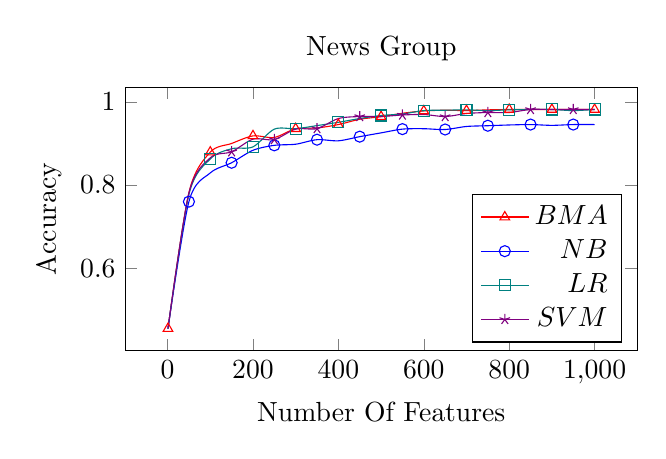
\begin{tikzpicture}
%[trim axis left, trim axis right]
\begin{axis}
[title=News Group,
ylabel=Accuracy,
xlabel=Number Of Features,
%cycle list name=color list,
cycle list={%
    red,blue,teal,violet,cyan,green!70!black,magenta,gray},
width=230pt,
height=140pt,
legend style={
	cells = {anchor = east},
	legend pos = south east,
	},
]
\addplot+[smooth, mark=triangle, mark repeat=2,mark phase=1] coordinates
%\addplot coordinates
        {(1,0.4545) (50,0.7818) (100,0.8791) (150,0.9000) (200,0.9182) (250,0.9145) (300,0.9355) (350,0.9373) (400,0.9455) (450,0.9582) (500,0.9645) (550,0.9727) (600,0.9782) (650,0.9800) (700,0.9791)  (750,0.9809) (800,0.9818) (850,0.9818) (900,0.9818) (950,0.9818) (1000,0.9818)};
\addplot+[smooth,mark=o,  mark repeat=2,mark phase=2] coordinates
%\addplot coordinates
        {(1,0.4545) (50,0.7600) (100,0.8291) (150,0.8536) (200,0.8836) (250,0.8955) (300,0.8982) (350,0.9091) (400,0.9064) (450,0.9164) (500,0.9255) (550,0.9345) (600,0.9355) (650,0.9336) (700,0.9409) (750,0.9427) (800,0.9445) (850,0.9455) (900,0.9436) (950,0.9455) (1000,0.9455)};
\addplot+[smooth,mark=square, mark repeat=2,mark phase=3] coordinates
%\addplot coordinates
{(1,0.4545) (50,0.7773) (100,0.8627) (150,0.8873) (200,0.8918) (250,0.9345) (300,0.9355) (350,0.9430) (400,0.9509) (450,0.9600) (500,0.9673) (550,0.9709) (600,0.9791) (650,0.9800) (700,0.9809) (750,0.9791) (800,0.9809) (850,0.9818) (900,0.9818) (950,0.9791) (1000,0.9818)};
\addplot+[smooth,mark=star, mark repeat=2,mark phase=4] coordinates
%\addplot coordinates
{(1,0.4545) (50,0.7806) (100,0.8655) (150,0.8800) (200,0.9103) (250,0.9095) (300,0.9345) (350,0.9358) (400,0.9600) (450,0.9648) (500,0.9648) (550,0.9685) (600,0.9697) (650,0.9648) (700,0.9721) (750,0.9745) (800,0.9745) (850,0.9818) (900,0.9818) (950,0.9818) (1000,0.9818) };
\legend{$BMA$,$NB$,$LR$,$SVM$}
\end{axis}
\end{tikzpicture}
\endpgfgraphicnamed
\end{center}
\caption{Classification Accuracy VS Number of Features}
\label{figure:7}
\end{figure}
%\end{sidewaystable}